\section{Method}\label{sec:method}

Being a system distributed across distinct computing platforms (a general
purpose computer; a network of microcontrollers), and software elements
serving a variety of purposes (server and client instances for transmission
and reception of networked audio and control data, plus a DSP algorithm), it is
important to consider each of these elements in detail.
In the subsections to follow, these elements are described;
finally an overview of the devised system is provided.

\subsection{The Networked Audio Server}\label{subsec:the-networked-audio-server}

TCP is, as described in \secref{subsubsec:protocols-systems}, a
connection-based, one-to-one protocol, so the JackTrip connection model enforces
a sort of pseudo-connectionfulness on the otherwise connectionless UDP.\
The result is a system which permits only unicast UDP transmission, and, for
multiple clients, must send a duplicate of the outgoing stream of audio
datagrams to each connected client.
A JackTrip server creates a sender and a receiver task for each client that
connects~\citep{caceres_jacktrip_2010};
notionally this entails, should enough clients connect, exhaustion of all
available network bandwidth;
as such, a unicast system does not meet the requirement of scalability as
described in \secref{subsec:distributed-audio-systems}.

A multicast NetJACK server was considered, but creating a client implementation
on what is essentially a bare-metal platform in the shape of the Teensy, was not
practical.
Further, due to a break in compatibility with Mac OS X systems, JACK-based
approaches are not truly cross-platform.\footnote{
    A successor to the defunct CoreAudio/JACK bridge has been proposed but
    remains unrealised:
    \url{https://github.com/jackaudio/jack-router/blob/main/macOS/docs/JackRouter-AudioServerPlugin.md}.
    This issue of course also affects the viability of the JackTrip-based
    approach.
}
Prioritising simplicity, in the form of an audio server having minimal
dependencies and a very specific task to achieve, attention was turned to the
design of a bespoke multicast networked audio server.

\subsubsection{Designing a Networked Audio Protocol}\label{subsubsec:designing-a-protocol}

Dependent on the intended application, and if assumptions can be made about
matters such as sampling rate and bit resolution, a \textit{no-protocol}
approach, such as described by Lopez-Lezcano~\citep{lopez-lezcano_jack_2012},
may be a viable one.
To improve the flexibility of the system and make it somewhat future-proof,
however, a simple packet header was devised.
Its structure is given in \lstref{listing:packet-header}.

\begin{codelisting}{
    Packet header structure,
    label=listing:packet-header,
    minted language=cpp,
    minted style=xcode,
    float=ht
}
    struct PacketHeader {
        uint16_t SeqNumber;
        uint8_t BufferSize;
        uint8_t SamplingRate;
        uint8_t BitResolution;
        uint8_t NumChannels;
    };
\end{codelisting}

The resulting six-byte header comprises a two-byte (unsigned 16-bit integer)
packet sequence number, to be incremented by the sender, plus four further bytes
describing the structure of the audio data in the packet.
Commonly-encountered sampling rates, and buffer sizes greater than 255, cannot
be represented by unsigned eight-bit integers, so these are supported by
enumerations inspired by those used by JackTrip.\footnote{
    \url{https://github.com/jacktrip/jacktrip/blob/v1.6.8/src/AudioInterface.h\#L56}
}

\texttt{BufferSize} describes the number of audio frames per packet\footnote{
    Often used interchangeably with the word \textit{sample}, a \textit{frame}
    represents the samples for all channels for a given sample instant;
    thus the number of frames in a network packet or audio buffer is the number
    of samples divided by the number of channels.
} as the $n$th power of 2; for example, the enumeration \texttt{BufferSizeT}
features a member \texttt{BufferSizeT::BUF16}; 16 being the fourth power of 2,
this member is assigned the number 4.
The \texttt{BitResolution} field could be used to transmit one of 8, 16, 24, or
32 as-is; there is a utility, however, when decoding a packet, in knowing the
number of \textit{bytes} per audio sample, so this is the number that is
represented, e.g. \texttt{BitResolutionT::BIT16} takes the value 2, the number
of bytes in a 16-bit integer.

For well-formed packets, \texttt{BufferSize} could be inferred from the size of
the packet (minus its header), divided by \texttt{NumChannels} and
\texttt{BitResolution}.
To permit scope for the detection of malformed packets, however, the expense
of an additional byte in the header was deemed a reasonable one.
Finally, the sequence number is intended as a means for a recipient to identify
the occurrence of packet loss, and will wrap around to zero every \num{65536}
packets.

One piece of information that is not stated in the packet header is the manner
in which audio samples in the packet should be interleaved.
The assumption taken \textemdash{} indeed, the same assumption used by JackTrip
\textemdash{} is that audio data is channel-interleaved, i.e.\ audio data
consists of a contiguous block of samples for one channel, followed by a block
for the next channel, and so on.

\subsubsection{Server Design}

\begin{figure}[ht]
    \centering
    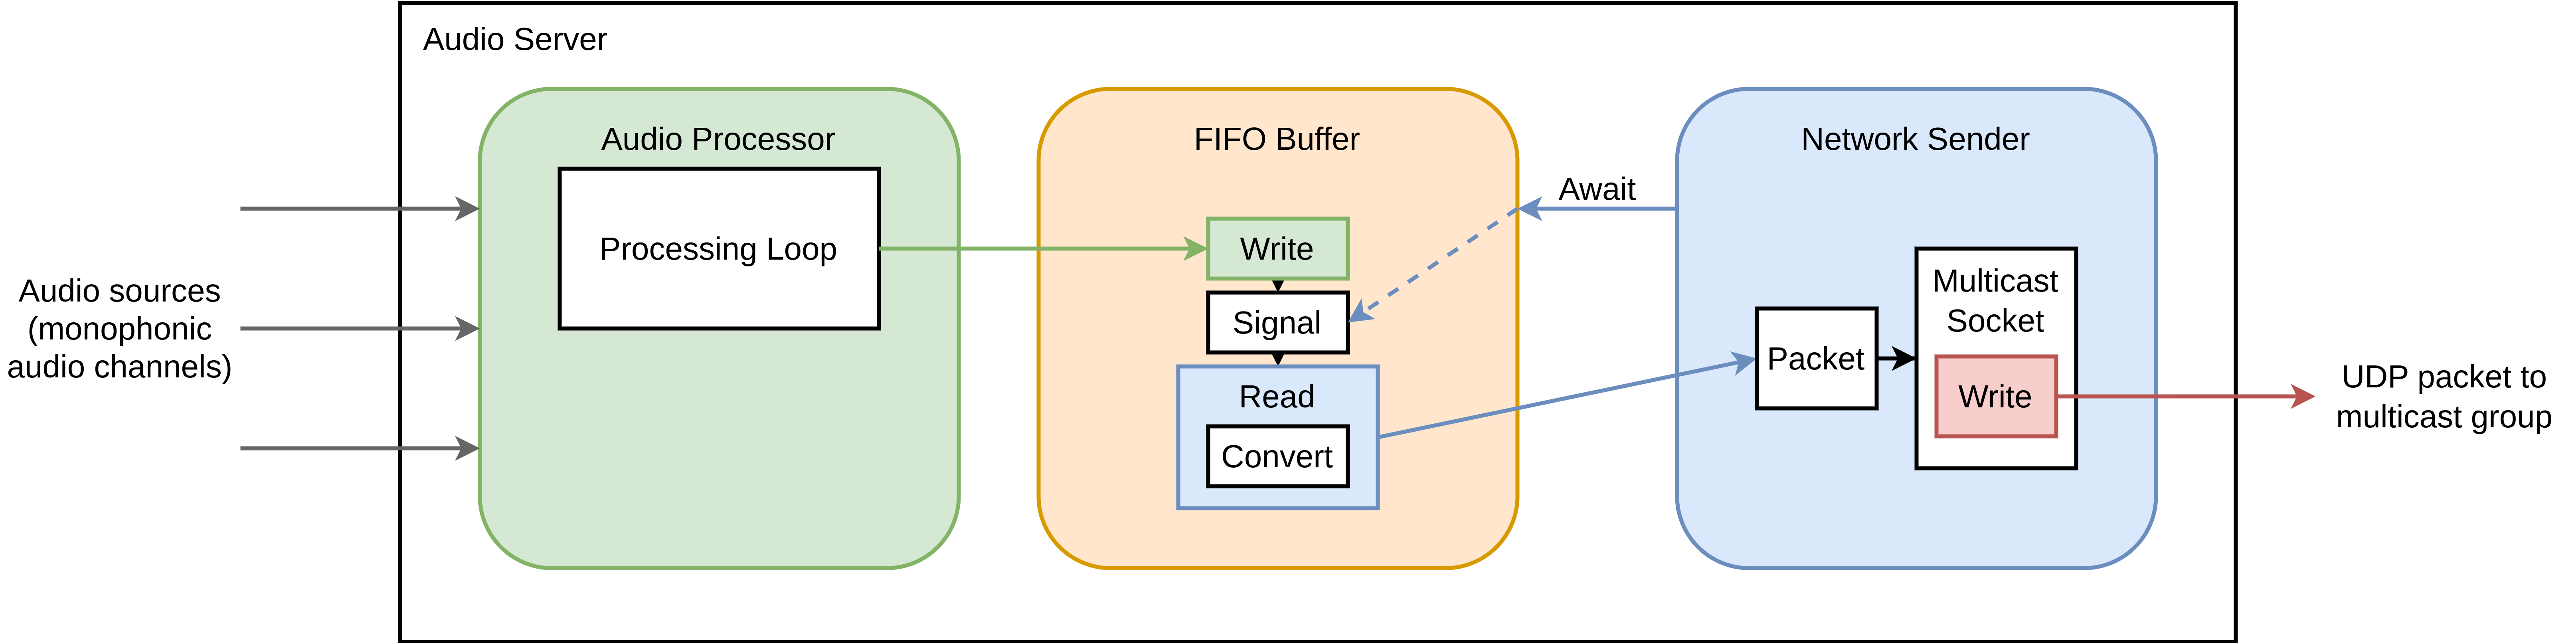
\includegraphics[width=\textwidth]{figures/audio-server}
    \caption{Overview of operation of the networked audio server.
    The network sender awaits notification of readiness to read samples from a
    first-in-first-out buffer of audio samples.
    The audio processor receives audio channels from a multichannel source
        (e.g. a DAW); at each iteration of its processing loop, it writes
        samples to the FIFO; upon write-completion, the FIFO sends a signal to
        the network sender that a block of samples is ready.
        Samples are converted to the desired bit resolution and byte order and
        bundled into a UDP packet which is then written to the network.}
    \label{fig:audio-server}
\end{figure}

The networked audio server was written in C++ using utility classes provided by
the JUCE framework for the development of audio applications.\footnote{
    JUCE 7.0.5 \url{https://github.com/juce-framework/JUCE}
}
The server is encapsulated as a class called \texttt{NetAudioServer},
which can be incorporated into any JUCE-based audio application;
initial development was conducted on a basic console application, and later work
targeted a DAW plugin comprising a consolidated audio server and wave field
synthesis controller.

The \texttt{NetAudioServer} instance expects to receive blocks of
multichannel audio from an audio application's main processing loop.
It sets up network \textit{sender} and \textit{receiver} execution threads, and
assigns a network socket to each; a socket is essentially a numerical identifier
for an
\textit{``endpoint for [network] communication''}~\citep{kerrisk_socket2_2023}
to which a type \textemdash{} \texttt{SOCK\_STREAM} for TCP on
\texttt{SOCK\_DGRAM} for UDP \textemdash{} can be assigned.
To avoid potentially blocking the audio application's main processing thread
with networking operations, upon receiving an audio block the server writes it
to an intermediate buffer \textemdash{} a first-in-first-out (FIFO) structure
\textemdash{} and signals the sender thread that a block is ready for
transmission.
The sender thread, which as been awaiting such a signal, then requests samples
from the FIFO; these are stored as contiguous channels of 32-bit floating point
samples and converted, when requested, to the bit resolution specified in a
packet header created when \texttt{NetAudioServer} is initialised.
Byte order, or \textit{endianness}~\citep{cohen_holy_1981}, is also specified as
part of this conversion.
Though network byte order is typically big-endian, or Most Significant Byte
(MSB) first, it was found that little-endian transmission meant that samples
could be decoded trivially at the client side.\footnote{
    Endianness is a thorny issue \textemdash{} just consider Danny Cohen's
    \textit{...Plea for Peace}~\citep{cohen_holy_1981}.
    To appeal momentarily to authority, JackTrip too transmits audio data (and
    port numbers, etc.) little-endian, ``network byte order'' notwithstanding.
}
Upon receiving the requested samples, the sender thread writes these to its
socket, which has been configured to connect to a UDP multicast group.
This process is illustrated in \figref{fig:audio-server}.

\codeinputlisting[float=ht]
{text}
{listings/audio-packet.txt}
{Network capture: ethernet frame containing a UDP audio packet}
{audio-packet}

\lstref{listing:audio-packet} shows an example network capture of an outgoing
audio packet.
Bytes \texttt{0x0000} to \texttt{0x0029} comprise the headers for the data link
(ethernet), network (IPv4), and transport (UDP) OSI layers including the
destination address: at position \texttt{0x001e}, the bytes \texttt{0xe004e004},
or \texttt{224.4.224.4}, a valid (and unassigned) UDP multicast address from the
second ad-hoc address block as specified in the IANA multicast address
assignment guidelines~\citep{meyer_iana_2010}.
The six subsequent bytes are the header inserted into the packet by
\texttt{NetAudioServer}.
In \lstref{listing:audio-packet} these are:
\begin{itemize}
    \item~\texttt{0x1cdf}: a sequence number (little-endian) of
    \numDec{7391};\footnote{Subscript 10 is employed here to indicate a decimal
    number.}
    \item~\texttt{0x04}: buffer size \num{4} corresponding with
    \texttt{BufferSizeT::BUF16};
    \item~\texttt{0x02}: sampling rate \num{2} corresponding with
    \texttt{SamplingRateT::SR44};
    \item~\texttt{0x02}: bit resolution \num{2} corresponding with
    \texttt{BitResolutionT::BIT16};
    \item~\texttt{0x02}: \num{2} audio channels.
\end{itemize}

Audio data begins at byte \texttt{0x0030}.
Since the header indicates that there are two channels of 16-bit audio, and a
buffer size of 16 frames, it is clear that the data for channel 1 encompasses
the 32 bytes from \texttt{0x0030} to \texttt{0x004f}, and channel 2 the
remaining bytes.

Here, channel 1 is a test signal, a unit amplitude-increment unipolar sawtooth
wave, i.e.\ a signal whose amplitude starts at zero, and increments by 1 at each
sample until it reaches the maximum value that a signed 16-bit integer may take
\textemdash{} \numDec{32767} \textemdash{} at which point it wraps around to
zero and repeats.
This test signal serves two important purposes.
First, its impulse-like behaviour once every \num{32768} samples (roughly
\qty{.74}{\s} at a sampling rate of \qty{44.1}{\kHz}) is useful for taking basic
synchronicity measurements, e.g.\ involving connecting two clients' audio
outputs to an oscilloscope.
Second, this numerically-predictable signal serves as a means to inspect the
integrity of the audio server algorithm, and to verify that the expected
sample interleaving and endianness is employed.
Inspecting the first sixteen samples of the first audio channel
it is evident that the amplitude values increment on a per-sample basis, and,
since it is the first byte that increases with each sample, that samples are
transmitted little-endian.

The purpose of the server's receiver thread is to poll its socket for traffic
reaching the multicast group from connected clients.
Clients are programmed to return a stream of packets of audio data to the
multicast group, and the receive thread uses the existence of a such a stream,
with a given origin IP address, to indicate the presence of a client at that
address.
If a client fails to return a packet for more than \qty{1}{\second} it is
considered disconnected.
Clients could announce their presence with any periodic UDP transmission, but
the possibility of returning audio data facilitates the measurement of client
synchronicity via transmission round trip times (see
\secref{subsec:technical-evaluation}).

\subsubsection{Transmission Considerations}\label{subsubsec:transmission-considerations}

Ethernet frames, and UDP datagrams by extension, are subject to size
limitations.
The maximum transmissible unit (MTU) of a transport medium is the limit on the
size of a packet that can be sent without fragmentation, i.e.\ without being
split into multiple sub-packets.
Two bytes are allocated to the `Total Length' field of the IPv4 header, which
suggests an MTU of $2^{16}-1=~$\num{65535} bytes;
in practice, however, the data link layer imposes a basic limit of \num{1500}
bytes on the payload of an ethernet
frame~\citep{schiavoni_alternatives_2013,ieee_ieee_2018}.

With the headers for the data link (Ethernet), network (IPv4), and transport
(UDP) layers accounted for, plus the audio header described above, in principle
\num{1452} bytes remain in each packet for audio data.
Assuming 16-bit resolution, and the transmission of one UDP packet per audio
buffer, data for up to 90 audio channels can be transmitted at a buffer size of
16 frames without fragmentation, or up to 45 channels at 32 frames.

\subsection{The Networked Audio Client}\label{subsec:networked-audio-client}

\begin{figure}[ht]
    \centering
    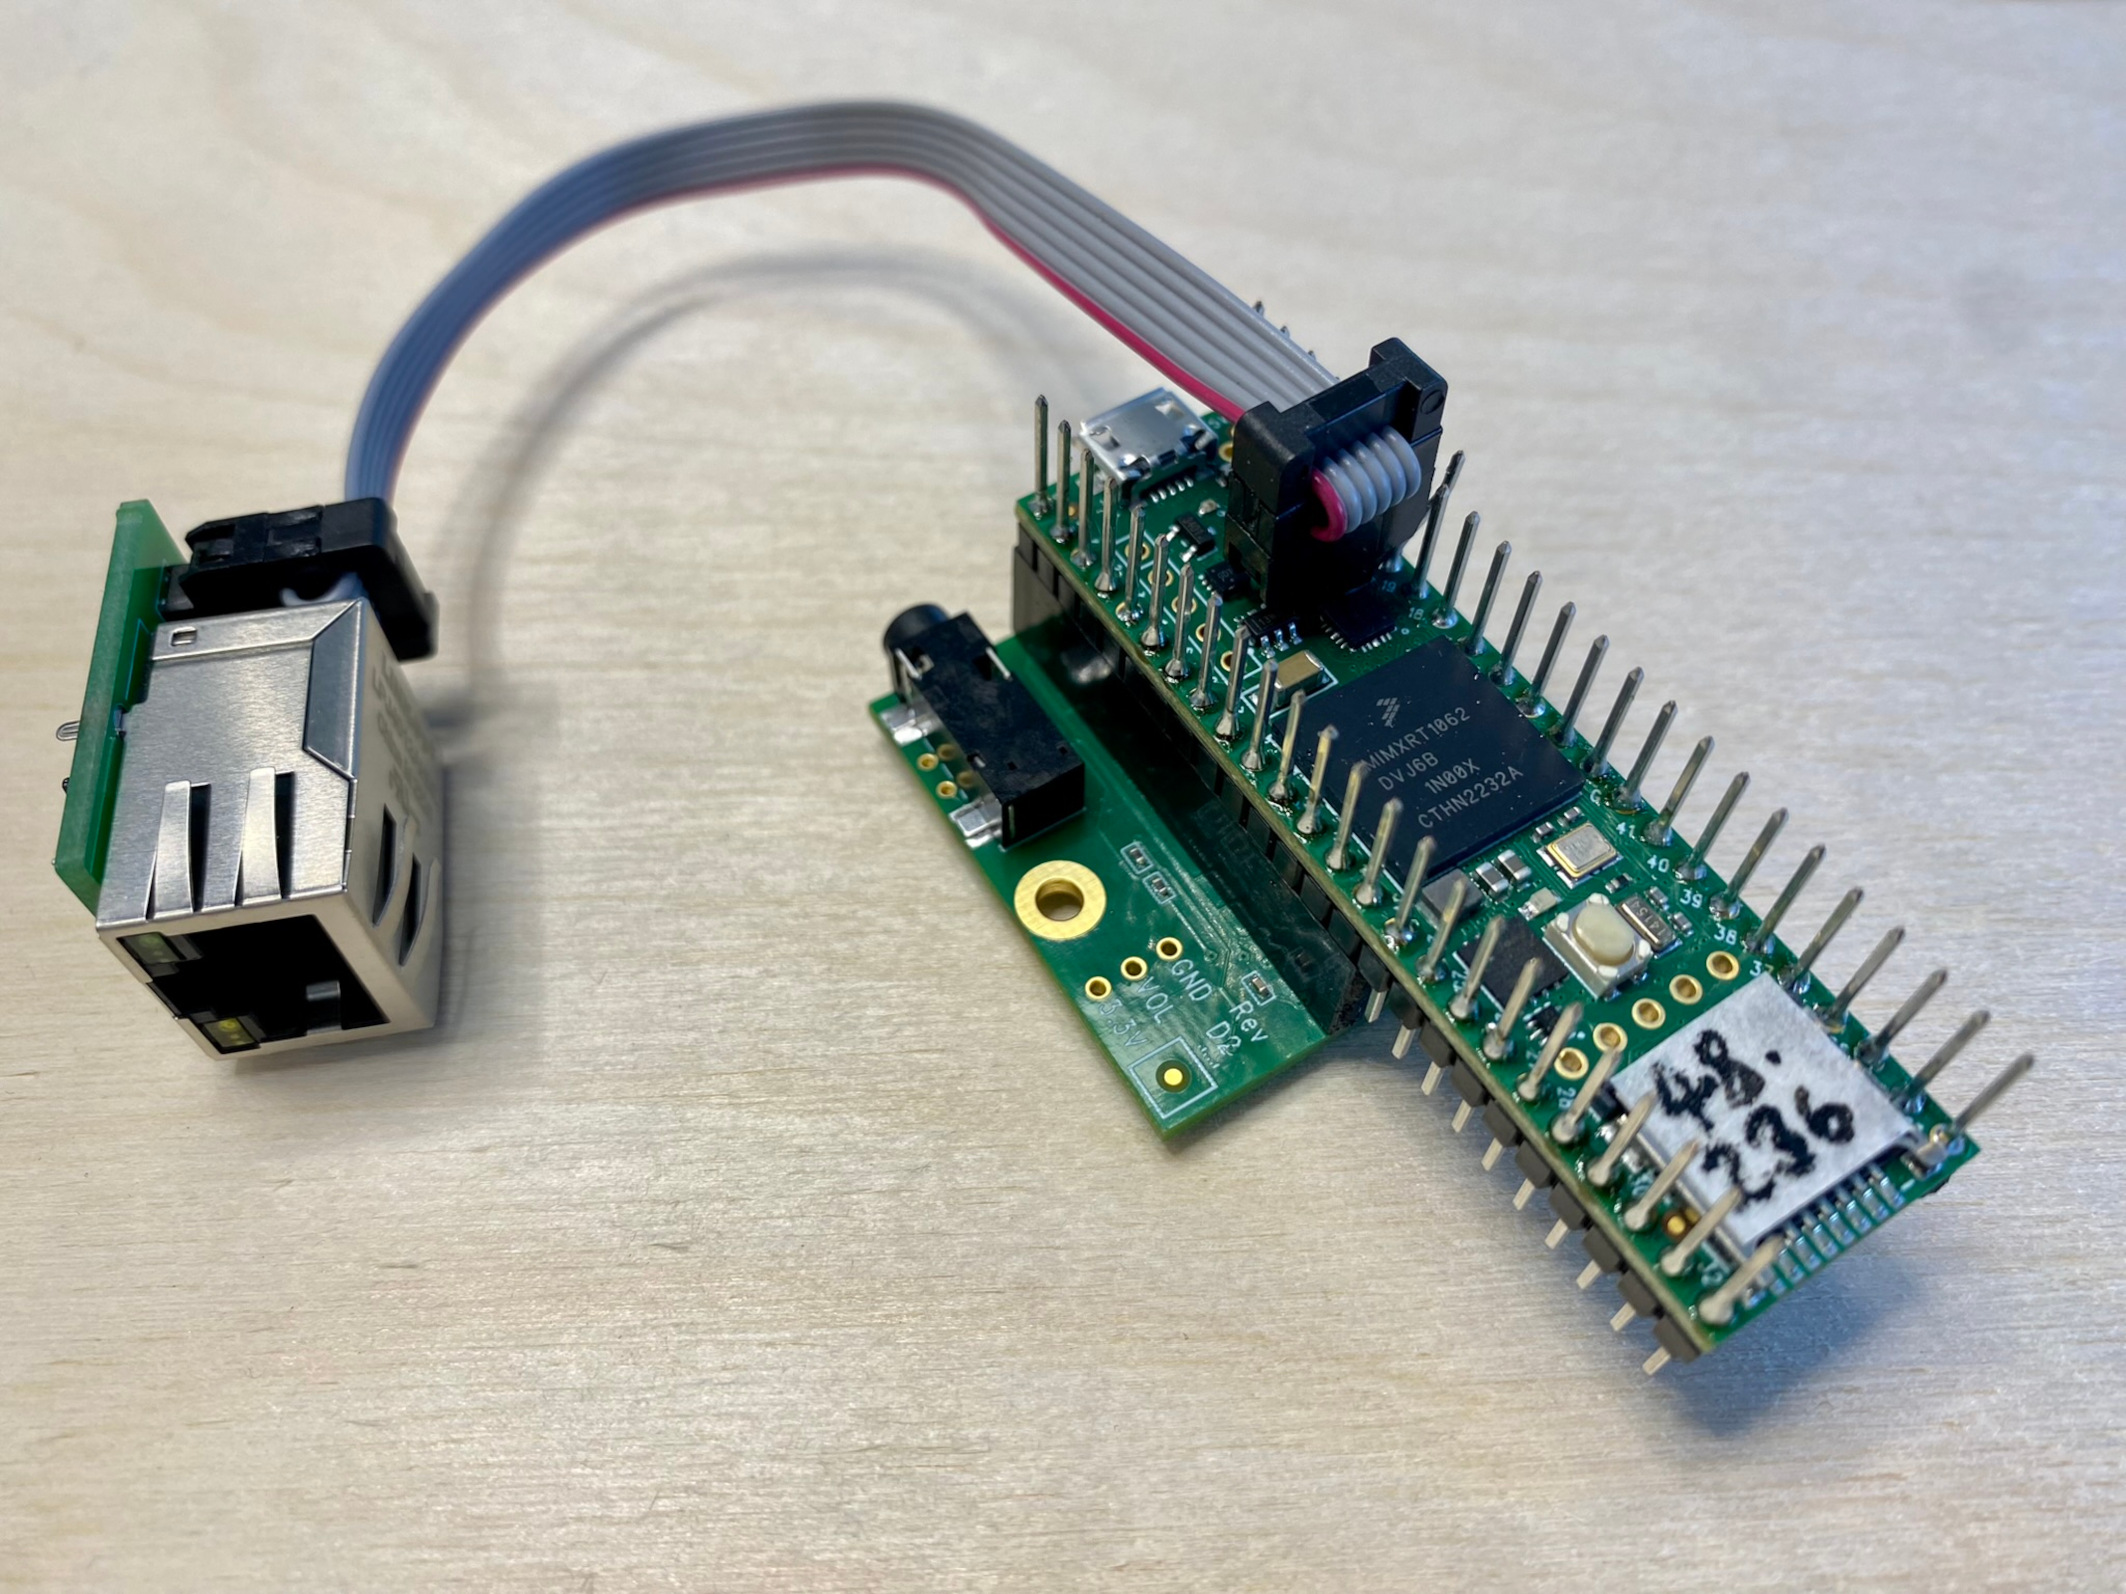
\includegraphics[width=.75\textwidth]{figures/module}
    \caption{A hardware module consisting of Teensy 4.1 microcontroller
        (labelled with the last two bytes of its serial number-derived IP address),
        connected via headers to an audio shield and via ribbon cable to an
        ethernet shield.}
    \label{fig:teensy}
\end{figure}

Unlike the networked audio server, which runs on a general purpose computer and
has access to threads of execution, which it can use to conduct related but
separate tasks that rely on some central resource (the FIFO buffer alluded to
above), the client implementation is designed to operate on a microcontroller
platform that has no operating system, and no native notion of threads.\footnote{
    There is in fact a non-core library, \textit{TeensyThreads}, that provides
    thread-like functionality. It was experimented with during development,
    but found to be incompatible with the interrupt-driven nature of the
    Teensy audio and networking libraries.
}

The task of the clients is threefold in nature:
\begin{enumerate}
    \item~to retrieve packets of audio data from the UDP multicast group;
    \item~to send a stream of audio data back to the multicast group, primarily
    to announce their connectivity;
    \item~to maintain, as far as possible, synchronous operation with the
    server, and (by extension) each other.
\end{enumerate}

To address the first two requirements, the client sets up a socket, which it
uses to both read from and write to the UDP multicast group.

The client was created as a C++ class named \texttt{NetJUCEClient}, an
implementation of the Teensy Audio Library class \texttt{AudioStream}.
\texttt{AudioStream} descendents must implement a method named
\texttt{update()}; this method is called at each audio hardware interrupt, and
is where an audio library class should perform operations on the current
audio buffer.
Networking operations are conducted from the method
\texttt{NetJUCEClient::loop}.\
Avoiding conflicts with audio functionality, this method is called from Teensy's
top level \texttt{loop()} function.
A valid Teensy program must define a function by this name, and it is called
repeatedly from the body of a non-terminating \texttt{while} loop throughout
operation.

\begin{figure}[ht]
    \centering
    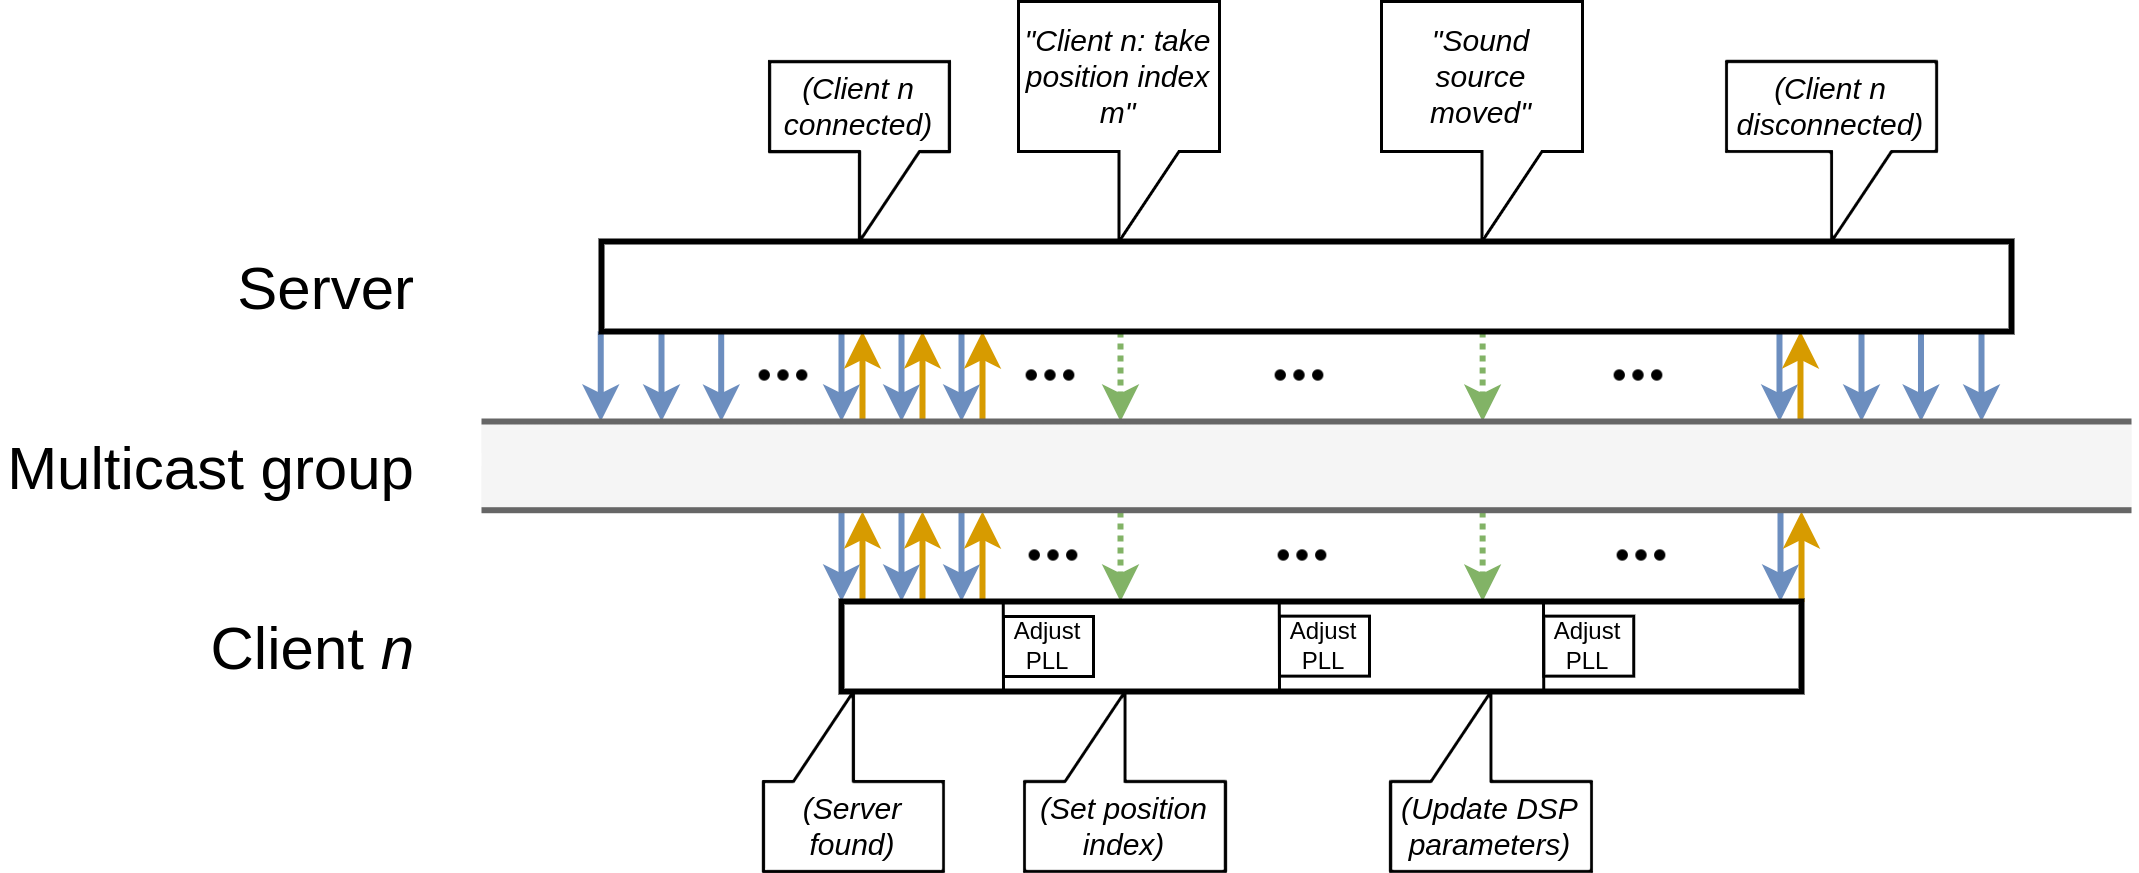
\includegraphics[width=\textwidth]{figures/timeline}
    \caption{
        Example timeline of interaction between the server and a client, via the
        UDP multicast group.
        Solid arrows indicate audio data being sent from the server to the
        multicast group;
        arrows with open heads indicate audio data being sent from the
        client back to the multicast group;
        arrows with dotted tails represent control data.
        Note that the server transmits to the multicast group irrespective of
        the presence of any client.
    }
    \label{fig:timeline}
\end{figure}

\begin{codelisting}{
    \texttt{loop} method of the networked audio client implementation,
    minted style=xcode,
    minted language=cpp,
    label=ls:njc-loop,
    float=h
}
    void NetJUCEClient::loop() {
        receive();

        checkConnectivity();

        send();

        adjustClock();
    }
\end{codelisting}

The two sets of operations are linked by way of an intermediate buffer, similar
to the FIFO employed by the server.
The client attempts to receive packets from, and, if it has generated a packet's
worth of audio data, send a packet to, the multicast group on each call to
\texttt{loop()}, with audio samples from incoming packets written to the
intermediate buffer (see \lstref{ls:njc-loop}).
The client also performs a periodic check for the presence of the server, and,
as described in \secref{subsubsec:client-sync}, makes adjustments to its audio
clock.
When multiple clients are present, there are consequently multiple streams of
audio packets reaching the multicast group.
To avoid ambiguity and unnecessary packet reads at the client side, server and
clients transmit audio data to the group on differing port numbers.

\begin{codelisting}{
    \texttt{update} method of the networked audio client implementation,
    minted style=xcode,
    minted language=cpp,
    label=ls:njc-update,
    float=h!
}
    void NetJUCEClient::update() {
        doAudioOutput();

        handleAudioInput();
    }
\end{codelisting}

On each audio interrupt, the client reads from the intermediate buffer to
produce samples for audio output.
It also takes samples reaching its audio inputs and adds those to a packet to be
sent to the multicast group at the earliest subsequent call to
\texttt{NetJUCEClient::loop} (\lstref{ls:njc-update}).
The client's inputs can receive samples from any Teensy Audio Library object to
which it has been connected programmatically;
for round-trip time measurements the client's audio outputs were routed back to
its inputs.
A timeline of client-server interaction is illustrated in \figref{fig:timeline}.

\subsubsection{Synchronicity with the Server}\label{subsubsec:client-sync}

Due to the influence of clock drift and transmission jitter, and since the
clients constitute a distributed system, with no direct knowledge of each other
and no authoritative source of time, their third task posed, without doubt,
the greatest challenge.
A two-pronged strategy was developed for addressing server-client and
inter-client timing discrepancies:

\textbf{Jitter Compensation:}
Similar to the approach taken in prior
work~\citep{rushton_microcontroller-based_2023}, clients monitored their
intermediate buffer for the difference between its write and read positions,
using a delay-locked loop to keep this difference within an interval of
one audio buffer's worth of frames.
This was achieved by way of setting thresholds for the read-write difference,
and adjusting the read-position increment if the difference fell beyond those
thresholds;
increasing the increment if the difference exceeded the high threshold;
decreasing it should the difference fall short of the low threshold.
This in turn entailed employing a fractional read-position, and interpolating
around it to achieve an appropriate sample value; essentially a form of adaptive
resampling.
For this purpose a cubic Lagrange interpolator was used; sample values for the
interpolator were converted from their 16-bit signed integer representation
to floating point numbers, interpolation conducted, and the resulting value
rounded to the nearest integer for output.

\textbf{Clock Drift Compensation:}
In the absence of an authoritative source of time, clients were set up to infer
the difference in rate between their own internal clock and that of the server
by comparing the rate of packet reception from the network to their internal
audio interrupt rate.
This was achieved by taking the ratio, over thirty-second intervals, of
packets written from the network to the intermediate buffer to blocks read
from the intermediate buffer for audio output.
This ratio was then used to calculate appropriate divisors to apply to the
\qty{24}{\MHz} master clock generated by a crystal oscillator on the Teensy,
adjusting the audio clock's phase locked loop (PLL) to produce an adjusted audio
sampling rate.
The aim of this approach was to minimise reliance on the adaptive resampler
described above, and ultimately encourage all clients to run at the same audio
rate as the server.

\subsection{The Audio Spatialisation Algorithm}\label{subsec:wfs-algorithm}

With some modifications, e.g.\ the possibility to specify speaker spacing
parametrically, the WFS algorithm
from~\citep{rushton_microcontroller-based_2023} was reused.
This algorithm was written in Faust and compiled to
a C++ class compatible with the Teensy Audio Library via Faust's
\texttt{faust2teensy} utility.
Hardware modules were connected to a general purpose computer via a USB hub
and the \texttt{tycmd} utility from the TyTools suite (see
\secref{subsec:hardware-platforms}) was used to ensure that all modules were
programmed with the same instructions.

As illustrated in \figref{fig:wfs_2}, producing the driving signal for a WFS
secondary source at position $\mathbf{x}$ entails applying a delay to an audio
signal $\sigink$, representing the $k$th virtual primary source.
This delay is based on the distance $r_k$ between $\mathbf{x}$ and the
desired virtual position of $\sigink$.
In its distributed form, the WFS algorithm, informed of the position in the
array of the two loudspeakers for which it is responsible, computes only the
delays for each primary source with respect to those two loudspeakers, i.e.\
for the $k$th virtual source, the $n$th hardware module computes
$r_{k,\mathbf{x}_{2n}}$ and $r_{k,\mathbf{x}_{2n+1}}$.
To reduce the computational burden placed on the hardware modules, specifically
with regard to memory, the length of the delay lines was reduced by discarding
the longitudinal component of $r_k$, leaving only the relative inter-speaker
delay.

For the WFS prefilter, $r_k$ was mapped to an inverse square law for
frequency-independent amplitude loss to the virtual medium of propagation, and
to the cutoff frequency of a two-pole lowpass filter defined by Faust's
\texttt{fi.lowpass} function.\footnote{
    \url{https://faustlibraries.grame.fr/libs/filters/\#filowpass}
}
Adopting a modified version of equation~\eqref{eq:driving-function}, the
driving function becomes:
\begin{equation}
    \label{eq:simple-driving-function}
    d_k(\bfx,t) = f(t, r_k) \ast \delta\left(t - \frac{r_k-y_k}{c}\right).
\end{equation}

\subsubsection{Modularity and Maximum Delay}

The reduction in the maximum delay length represented by the subtraction of
the longitudinal distance component in
equation~\eqref{eq:simple-driving-function} is essential for the viability of
the system.
As capable a platform as Teensy 4.1 is, as described in
\secref{subsec:hardware-platforms}, it is limited in terms of memory.
This in turn places limits on the lengths of delay lines that it can compute,
a matter exacerbated if there are many such delays to consider, such as in the
case of a WFS implementation with numerous virtual sound sources.
Each hardware module must compute two delay lines for each virtual source, one
for each of its output channels, the maximum length of which (depending on
the position of a given module in the speaker array) corresponds, after removal
of the longitudinal component, to the width of the speaker array.
It was observed that, for eight virtual sources and eight hardware modules,
the maximum speaker spacing permissible lay at around \qty{.4}{\m},
corresponding with a speaker array of maximum width 15 $\times$ 0.4 =
\qty{6}{\m}, equating to a maximum delay of $\sim$\qty{17}{\ms} or
approximately 795 samples at a sampling rate of \qty{44.1}{\kHz}.
The matter has not been rigorously tested, but nonetheless the presumption is
that this places significant limits on the modularity of the system.
Teensy's memory capacity can be extended by attaching up to two inexpensive
PSRAM chips for a further \qty{16}{\mega\byte} of memory.
These chips must be soldered onto the Teensy board, however, and the suitability
of such additional memory for rapid access, such as is required in an audio DSP
algorithm, remains to be investigated.

\subsubsection{Controlling the WFS Algorithm}

Parameter values are delivered to the Faust algorithm in the form of Open Sound
Control (OSC) messages.
OSC control data, describing virtual sound source positions, speaker spacing,
and informing clients of their position in the speaker array, is bundled into
UDP packets and delivered by the server to the multicast group for all clients
to consume.
Source positions are described as coordinates in a two-dimensional plane, with
$x$ and $y$ components, each normalised to the range $[0,1]$, transmitted
separately.
The width of the speaker array is inferred from the speaker spacing (in
metres), multiplied by the number of speaker-intervals in the array, i.e.\ one
fewer than the number of speakers.
For the proposed implementation, the number of speakers is known to the server
and clients at compile time; with further development this could be made
specifiable at runtime.
Similarly, at the time of writing, the longitudinal depth of the virtual
sound field is hard-coded into the clients and will be generalised in a future
iteration of the system.

\codeinputlisting[float=h]
{text}
{listings/control-data-packet.txt}
{Network capture: ethernet frame containing a UDP control data packet}
{control-data-packet}

\lstref{listing:control-data-packet} demonstrates an example control data
packet, an OSC bundle containing one message.
This message has address \texttt{/source/0/x}, indicating that it refers to the
$x$-coordinate of the zeroth sound source, providing a value in the form of a
big-endian 32-bit floating point number, \texttt{0x3d1b5fa2}, approximately
\numDec{0.038}.

\subsection{System Overview}\label{subsec:system-overview}

The proposed system being composed of multiple hardware and software components,
it is worthwhile to summarise the nature of these components and the
interactions between them.

\subsubsection{Hardware Setup}

The networked audio server runs on a general purpose computer.
During the development and testing of this project, that computer was an ASUS
G513R Notebook PC, with an AMD Ryzen 7 6800H processor with a clock
speed of \qty{3.2}{\GHz}.
For the majority of development, the computer's internal sound card was used;
for testing and evaluation, it was connected to a Steinberg UR44C USB audio
interface, the hope being that external hardware would provide more consistent
audio interrupt timing, thus minimising jitter originating at the server.

The computer was connected via CAT6 ethernet cable to an eight-port ethernet
switch (D-Link DGS-108GL).
For evaluation, and to support a total of eight networked audio clients, this
switch was daisy-chained to an additional switch (D-Link DES-1008D).
Teensy 4.1 hardware modules, assembled as per \figref{fig:teensy}, were
connected via CAT6 ethernet cables to available ports on the ethernet switches.
Hardware modules were powered by a combination of a seven-port USB hub, plus,
for the eighth module, a USB mains socket.
The two audio outputs of each hardware module were connected to M-Audio BX5
loudspeakers.

\subsubsection{Software System}\label{subsubsec:software-system}

\begin{figure}[ht]
    \centering
    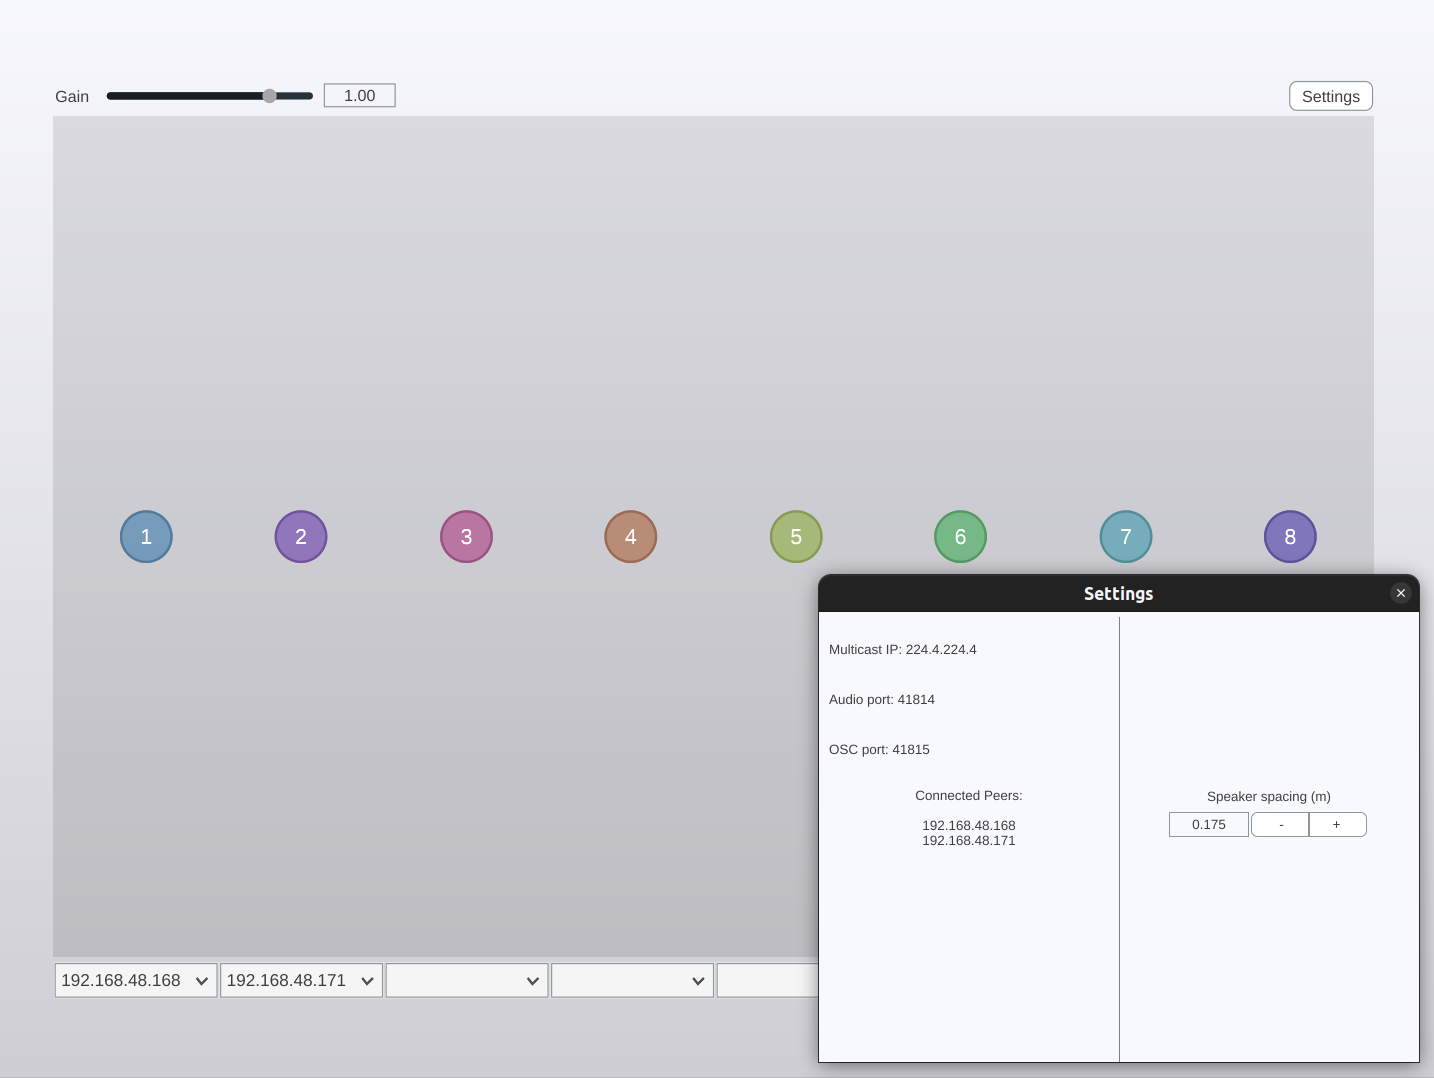
\includegraphics[width=\textwidth]{figures/plugin}
    \caption{
        User interface for the WFS controller DAW plugin, with modal
        settings window visible.
        The interface consists of an X/Y control surface, with eight nodes
        representing the coordinates, normalised to $x,y \in [0,1]$, of sound
        sources in a virtual sound field.
        Dropdown menus at the bottom of the interface correspond with hardware
        module positions in the loudspeaker array; there are eight such menus
        in total, each associated hardware module producing output for two
        loudspeakers.
        The settings window facilitates specifying the speaker spacing, and
        shows a list of connected network peers.
    }
    \label{fig:plugin-interface}
\end{figure}

Server-side, the software system consists of a VST plugin running in Reaper
digital audio workstation software.\footnote{\url{https://reaper.fm/}}
The plugin comprises the networked audio server, receiving monophonic audio
sources in the form of audio or instrument tracks in the DAW, plus a control
data server, commanded either by parameter automation via the DAW, or manually
via a graphical user interface (see \figref{fig:plugin-interface}).
The audio and control data servers send streams of UDP packets to a UDP
multicast group.

Client-side software connects to the multicast group and reads UDP packets
containing audio and control data from the server.
These streams are delivered to the Faust-based WFS algorithm, with audio
streams processed according to the control parameters of virtual sound source
positions and speaker spacing.
The WFS algorithm produces driving signals for each of the two output channels
of the hardware module on which it is running.
Additionally, the client-side networked audio client returns a stream of audio
data to the multicast group, to be consumed by the server.

Code for the server and client software components can be found at
\url{https://github.com/hatchjaw/netjuce} and
\url{https://github.com/hatchjaw/netjuce-teensy} respectively.
